\section{evaluation}
\label{sec:evaluation}

In this section we introduce the evaluation result of our prototype implementation in Amazon EC2 public cloud.
The cloud environment is shown as Table.\ref{evaluation:amazon_environment}
\begin{table}[h]
\centering
\begin{tabular}{|c|c|}
\hline
\cellcolor{lightgray} Region				&		Tokyo		\\
\hline
\cellcolor{lightgray} Instance Type		&		m3.xlarge	\\
\cellcolor{lightgray} vCPUs				&		4			\\
\cellcolor{lightgray} ECUs				&		13			\\
\cellcolor{lightgray} Memory				&		15GiB		\\
\cellcolor{lightgray} Instance Storage	&		2*40GB(SSD)	\\
\cellcolor{lightgray} Network Performance	&		High		\\
\end{tabular}
\caption{evaluation environment}
\label{evaluation:amazon_environment}
\end{table}

\begin{table}[th]
\centering
\begin{tabular}{|c|p{150pt}|}
\hline
CPU					&		Intel\textregistered Core\texttrademark i7-3770K CPU @ 3.50GHz\\\hline
Memory				&		16GB\\\hline
Storage				&		Crucial m4 CT256M4SSD3 (256GB, mSATA)(Peak read: 500 MB/s, Peak write:260MB/s)*8\\\hline
RAID Card 			&		Adaptec ASR-7805Q Single\\\hline
RAID				&		Raid 0\\
\hline
\end{tabular}
\caption{storage environment}
\label{evaluation:storage_environment}
\end{table}

Here vCPUs means the number of virtual CPU in instance, and one ECU provides the equivalent CPU
capacity of a 1.0-1.2GHz 2007 Opteron or 2007 Xeon processor.

For the storage system, we used a machine inside our lab, the details is shows in
Table.~\ref{evaluation:storage_environment}.

All the compute nodes, I/O nodes and master node connect with interconnection network inside Amazon
EC2, and mount storage system by sshfs\cite{sshfs} via Internet.

We use gxp\cite{gxp} to distribute work flow over compute nodes.

\subsection{One User Performance}

\begin{figure}
\centering
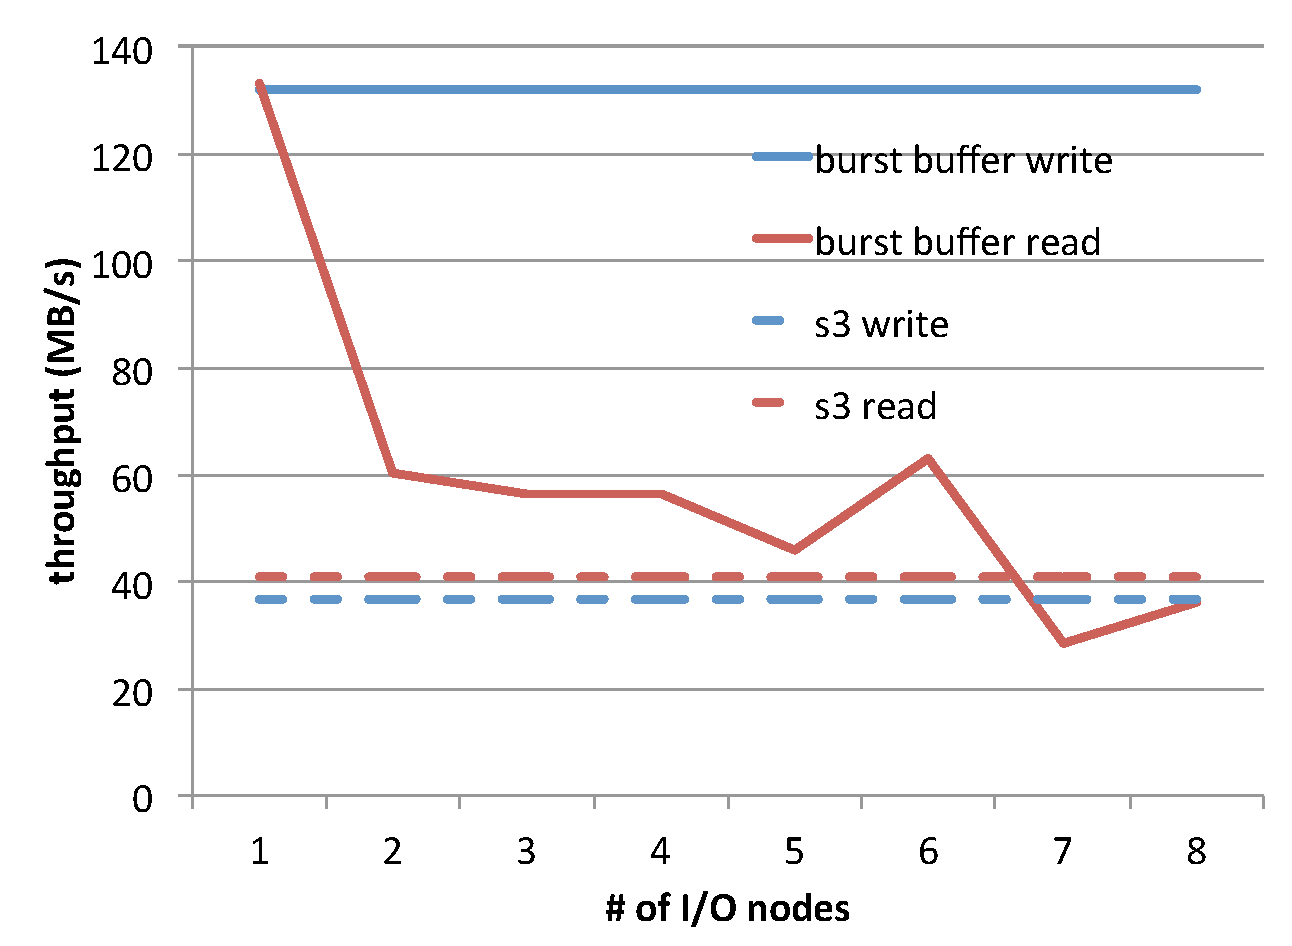
\includegraphics[width=8.5cm]{img/one_client.pdf}
\caption{One User Performance}
\label{evaluation:one user performance}
\end{figure}

First we measure the performance of our prototype for only one user, and show how our system
will affect one user performance.
In this experiment, the number of client is fixed to one, and measure
the sequential read and write performance for different number of I/O nodes.
All I/O data are distributed among all I/O nodes.
Figure~.\ref{evaluation:one user performance} shows one user performance.
As we know, one thread I/O is difficult to achieve the full throughput on Internet, we can see from
Figure.~\ref{evaluation:one user performance} that without I/O node, applications can only achieve a
throughput under 20MB/s in reading and under 80MB/s in writing.

However by using our system the read throughput increasing as the number of I/O nodes, and can
achieve about 8 times faster than the throughput without I/O nodes.
For writing throughput, the interconnection throughput is different from Internet throughput, it can
achieve full throughput even with one thread, but the throughput is limited by the client node
throughput which is also 1Gbps(135MB/s).

\subsection{Multiple Users Performance}

\begin{figure}
\centering
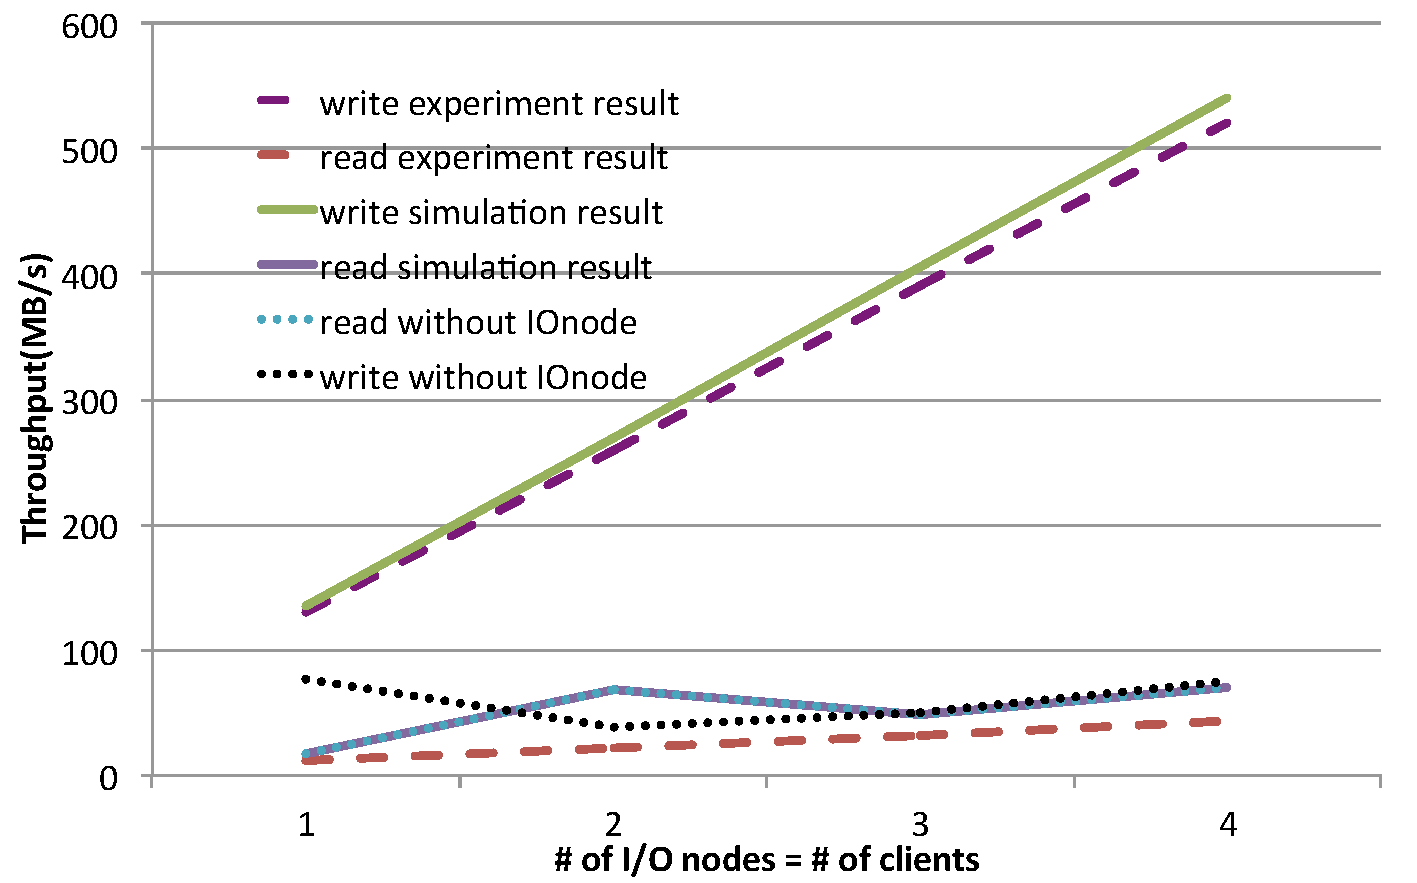
\includegraphics[width=8cm]{img/multiple_client.pdf}
\caption{Multiple User Performance}
\label{evaluation:multiple user performance}
\end{figure}

In the second experiment, we measured the throughput of multiple clients.
It shows the overall throughput the whole system can achieve.
To simplify the experiment, we assume that one client connects to only one I/O nodes, and one I/O
nodes buffer all the I/O data for a client.
Figure.~\ref{evaluation:multiple user performance} shows the overall throughput of the whole system.
First we see the result of traditional solution in which all compute nodes connect to shared storage
and read write data concurrently.
However, since the connection bandwidth of shared storage, which is the Internet bandwidth is only
1Gbps, the overall throughput grows at first, and quickly hit the limitation.

Then we look at the result using our system.
Since all the data are stored on the shared storage, and need to
be transferred via Internet, the read throughput doesn't change by using I/O nodes.
However when we look at the write throughput, it shows a strong scalability, and achieved 7 times
improvement with only 4 I/O nodes.

\subsection{Simulation for Applications}

\begin{figure}
\centering
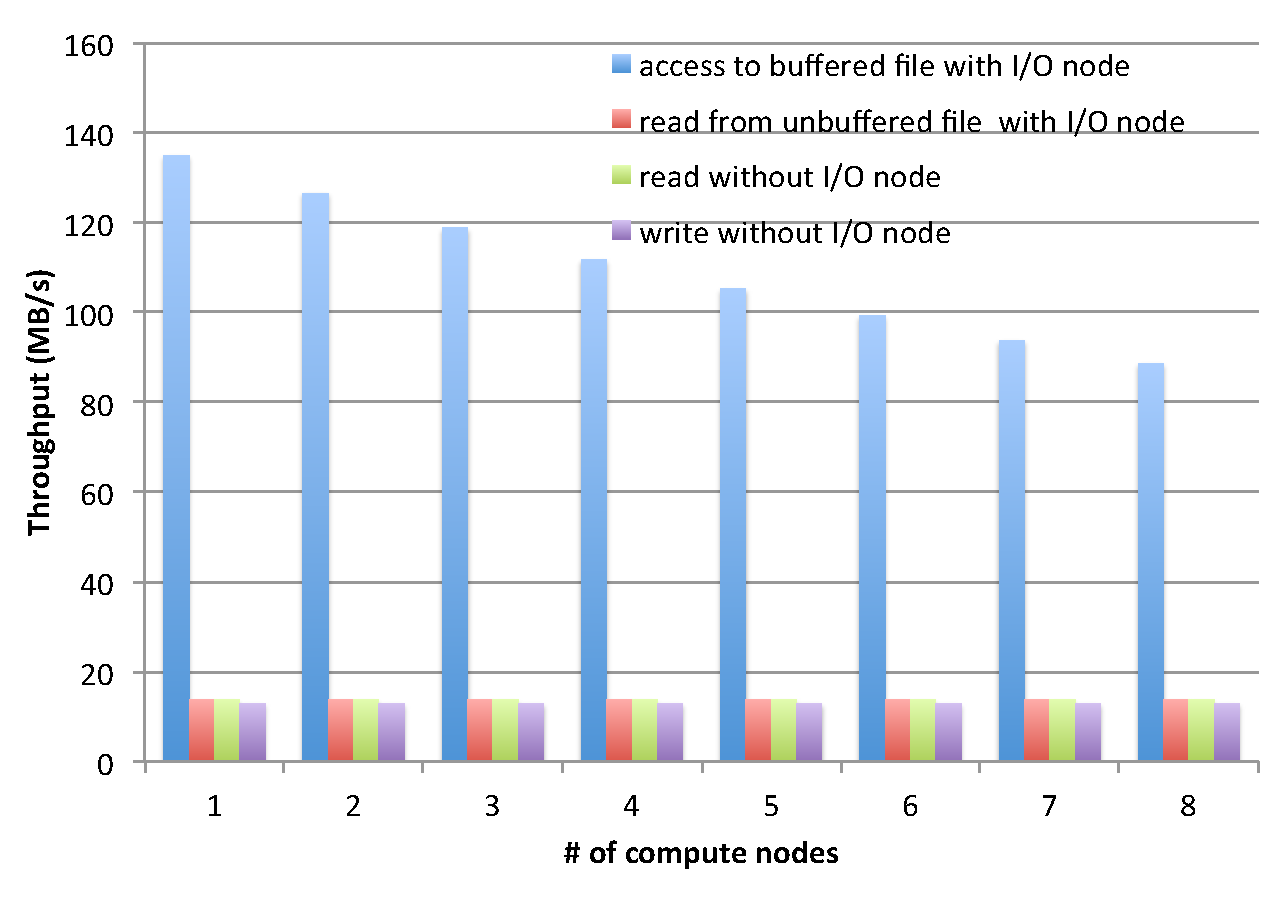
\includegraphics[width=8cm]{img/simulation_throughput}
\caption{read write throughput of one compute node with 8 I/O nodes}
\label{evaluation:simulation throughput}
\end{figure}

\begin{table}
\centering
\begin{tabular}{|c|c|c|c|}
\hline
						&	Montage		&		Pov Ray		&		Supernovae		\\\hline
total I/O size(MB)		&	2132.437508	&		748.916378	&		5203.214882		\\\hline
total read size(MB)		&	1558.082295	&		681.081228	&		3283.723596		\\\hline
total write size(MB)	&	574.355213	&		67.83515	&		1919.491286		\\\hline
read locality size(MB)	&	1500.107713	&		678.155227	&		2429.888509		\\\hline
compute time (s)		&	18.680705	&		1150.97979	&		1351.987268		\\
\hline
\end{tabular}
\caption{Applications Execution detail}
\label{evaluation:application execution detail}
\end{table}

\xtq{define what and why is $T$}

 In this section, we simulate the execution of the three applications shown in
 Table.~\ref{background:work flow applications} on our prototype system.
 Since the I/O from other compute nodes will affect the I/O throughput of one compute node,
 in order to simulate the execution of different number of compute node and find the throughput of
 one compute node.
% First we make several assumptions:
% \begin{itemize}
%   \item Master distribute I/O data of applications over all I/O nodes evenly, and applications
%   evenly access I/O data.
% %  \item All I/O data are evenly distributed over all I/O nodes.
% %  \item Applications access all data evenly.
%   \item The I/O bandwidth between compute nodes and I/O nodes is always $T$.
%   \item If multiple compute nodes connect to a single I/O node, they can share the bandwidth of the
%   I/O node equally.
% %  \item Multiple compute nodes can share the throughput of I/O nodes equally.
% \end{itemize}
% 
% As we assume that multiple compute nodes can share the throughput of I/O nodes equally, one
% compute node can achieve $\frac{1}{i+1}$ of the total throughput of I/O node when shared with other
% $i$ compute node, so we can sum it up and get the final throughput:
% \begin{equation}
% \text{Throughput}=\sum_{i=0}^{n-1} \frac{\text{rate}_i}{i+1} \times T
% %\text{T}=\frac{T}{e} 
% %e=1+\frac{n-1}{m}
% \end{equation}
% 
% With above assumptions, then we can calculate the rate of one compute node shared one I/O node with
% other $i$ compute node with total $m$ I/O nodes and $n$ compute node as
% 
% \begin{equation}
% \text{rate}_i=\frac{\dbinom{n-1}{i}(m-1)^{n-i-1}}{m^{n-1}}
% \end{equation}


Figure.~\ref{evaluation:simulation throughput} shows the one compute node throughput with 8 I/O
nodes for different number of compute nodes, since for buffered file, compute nodes can assess these
files from I/O nodes, the read and write throughput are both equal to I/O nodes throughput.
Since we buffer all the output data, there is only read case can access to unbuffered file which
can only achieve a low throughput.

Table~.\ref{evaluation:application execution detail} shows the execution detail of the three
applications.


\begin{figure}
\centering
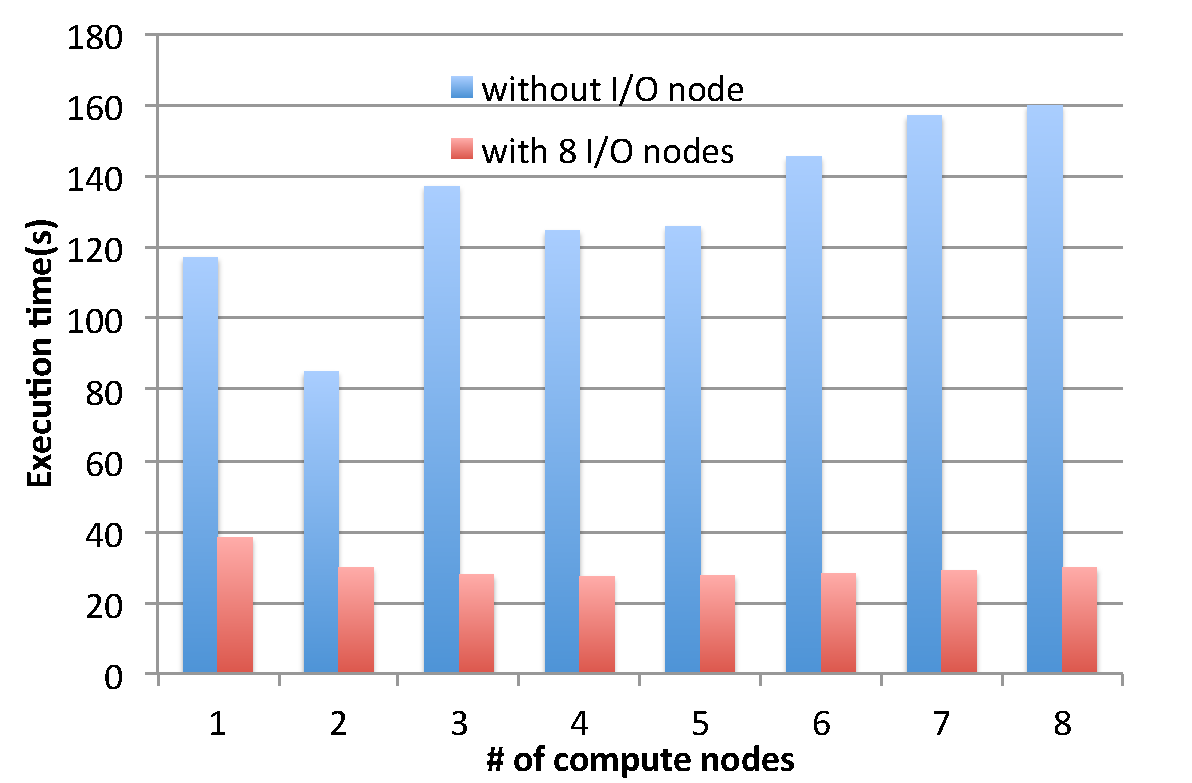
\includegraphics[width=8cm]{img/simulation_montage}
\caption{simulation result of montage}
\label{evaluation:simulation result montage}
\end{figure}


\begin{figure}
\centering
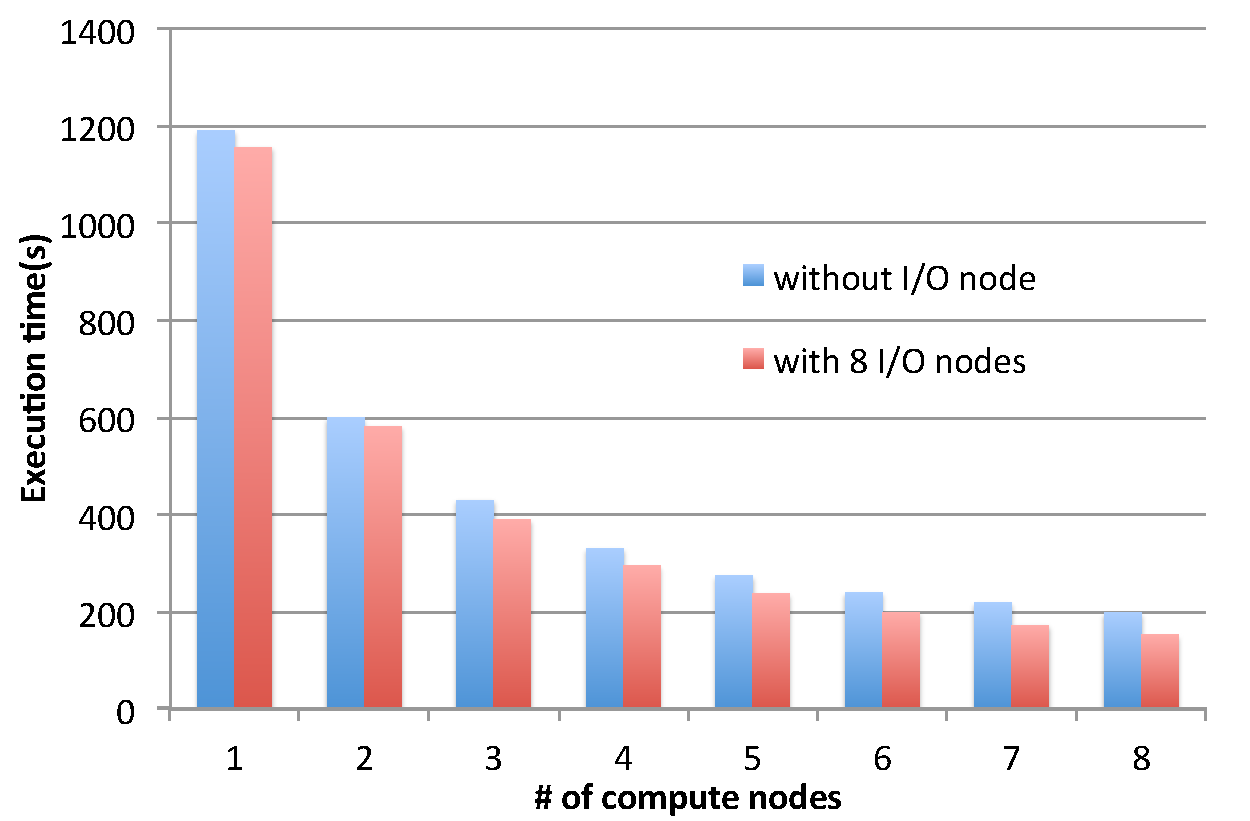
\includegraphics[width=8cm]{img/simulation_povray}
\caption{simulation result of pov ray}
\label{evaluation:simulation result pov ray}
\end{figure}

\begin{figure}
\centering
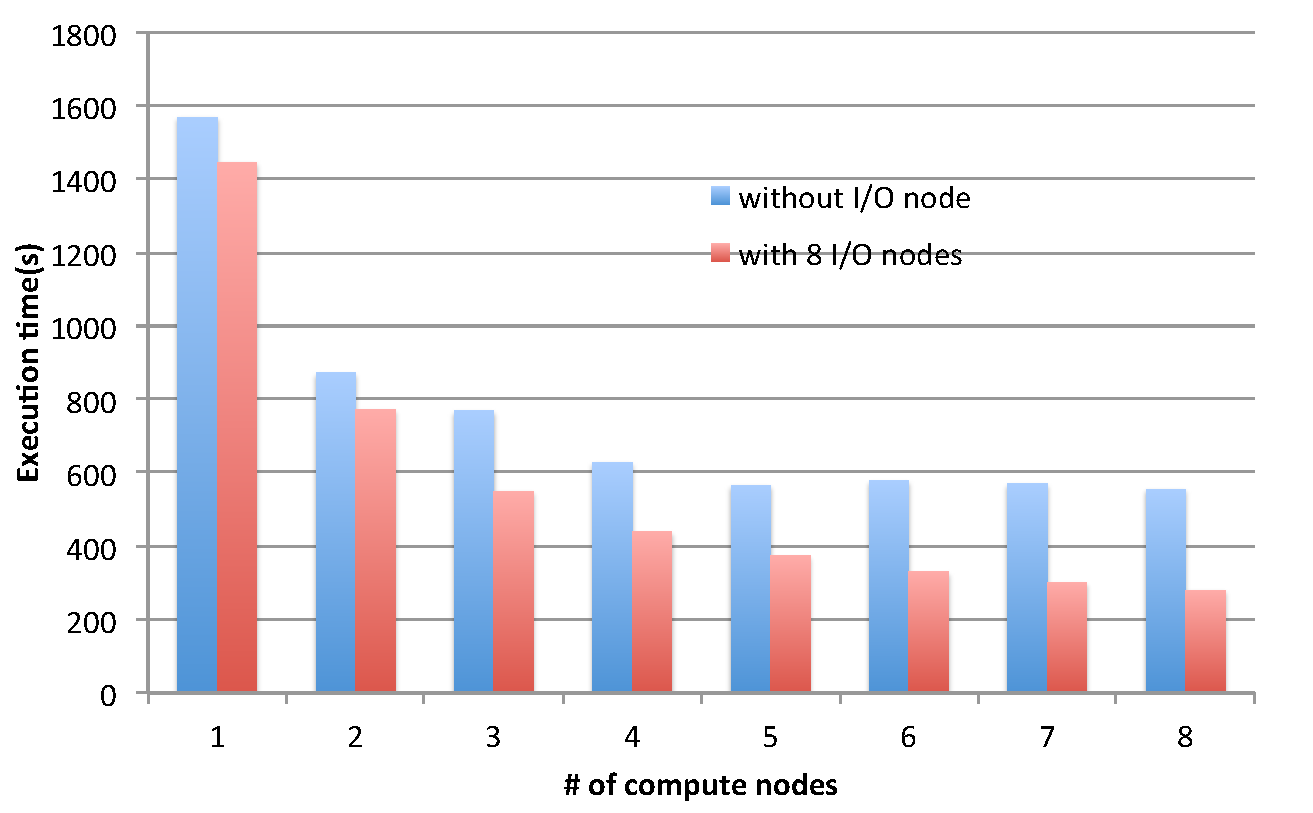
\includegraphics[width=8cm]{img/simulation_supernovae}
\caption{simulation result of supernovae}
\label{evaluation:simulation result supernovae}
\end{figure}

As we can see from Figure.~\ref{evaluation:simulation result montage},\ref{evaluation:simulation
result pov ray},\ref{evaluation:simulation result supernovae}, by using our system, all three
applications achieved a high improvement.
Among them, Montage has the largest improvement since it I/O a lot but do not do much
computation.
On the contrary, Pov Ray has a heavy computation, and a small I/O size, and gets a small performance
improvement by using our system.
